%%
%% This is file `sample-sigconf.tex',
%% generated with the docstrip utility.
%%
%% The original source files were:
%%
%% samples.dtx  (with options: `sigconf')
%% 
%% IMPORTANT NOTICE:
%% 
%% For the copyright see the source file.
%% 
%% Any modified versions of this file must be renamed
%% with new filenames distinct from sample-sigconf.tex.
%% 
%% For distribution of the original source see the terms
%% for copying and modification in the file samples.dtx.
%% 
%% This generated file may be distributed as long as the
%% original source files, as listed above, are part of the
%% same distribution. (The sources need not necessarily be
%% in the same archive or directory.)
%%
%%
%% Commands for TeXCount
%TC:macro \cite [option:text,text]
%TC:macro \citep [option:text,text]
%TC:macro \citet [option:text,text]
%TC:envir table 0 1
%TC:envir table* 0 1
%TC:envir tabular [ignore] word
%TC:envir displaymath 0 word
%TC:envir math 0 word
%TC:envir comment 0 0
%%
%%
%% The first command in your LaTeX source must be the \documentclass
%% command.
%%
%% For submission and review of your manuscript please change the
%% command to \documentclass[manuscript, screen, review]{acmart}.
%%
%% When submitting camera ready or to TAPS, please change the command
%% to \documentclass[sigconf]{acmart} or whichever template is required
%% for your publication.
%%
%%
\documentclass[sigconf]{acmart}

%%
%% \BibTeX command to typeset BibTeX logo in the docs
\AtBeginDocument{%
  \providecommand\BibTeX{{%
    Bib\TeX}}}

%% Rights management information.  This information is sent to you
%% when you complete the rights form.  These commands have SAMPLE
%% values in them; it is your responsibility as an author to replace
%% the commands and values with those provided to you when you
%% complete the rights form.
\copyrightyear{2023}
\acmYear{2023}
\setcopyright{rightsretained}

%% These commands are for a PROCEEDINGS abstract or paper.
\acmConference[SIGSPATIAL '23]{The 31st ACM International Conference on Advances in Geographic Information Systems}{November 13--16, 2023}{Hamburg, Germany}
\acmDOI{10.1145/3589132.3629970}

%%
%%  Uncomment \acmBooktitle if the title of the proceedings is different
%%  from ``Proceedings of ...''!
%%
%%\acmBooktitle{Woodstock '18: ACM Symposium on Neural Gaze Detection,
%%  June 03--05, 2018, Woodstock, NY}
% \acmPrice{15.00}
\acmBooktitle{The 31st ACM International Conference on Advances in Geographic Information Systems (SIGSPATIAL '23), November 13--16, 2023, Hamburg, Germany}
\acmISBN{979-8-4007-0168-9/23/11}

%%
%% Submission ID.
%% Use this when submitting an article to a sponsored event. You'll
%% receive a unique submission ID from the organizers
%% of the event, and this ID should be used as the parameter to this command.
%%\acmSubmissionID{123-A56-BU3}

%%
%% For managing citations, it is recommended to use bibliography
%% files in BibTeX format.
%%
%% You can then either use BibTeX with the ACM-Reference-Format style,
%% or BibLaTeX with the acmnumeric or acmauthoryear sytles, that include
%% support for advanced citation of software artefact from the
%% biblatex-software package, also separately available on CTAN.
%%
%% Look at the sample-*-biblatex.tex files for templates showcasing
%% the biblatex styles.
%%

%%
%% The majority of ACM publications use numbered citations and
%% references.  The command \citestyle{authoryear} switches to the
%% "author year" style.
%%
%% If you are preparing content for an event
%% sponsored by ACM SIGGRAPH, you must use the "author year" style of
%% citations and references.
%% Uncommenting
%% the next command will enable that style.
%%\citestyle{acmauthoryear}


%%
%% end of the preamble, start of the body of the document source.
\begin{document}

%%
%% The "title" command has an optional parameter,
%% allowing the author to define a "short title" to be used in page headers.

\title{Diving into Supraglacial Lakes Detection: a Deep Semantic Segmentation Approach}

%% Diving into Supraglacial Lakes Detection: a Deep Semantic Segmentation Approach
%% A Deep Semantic Segmentation Dive into Supraglacial Lakes from Satellite Imagery (draft title)
%% Diving into Supraglacial Lakes Detection: a Semantic Segmentation using Satellite Images Approach
% TODO: Possible other title ideas:
% - Deep Dive into Supraglacial Lakes from Satellite Imagery
% - Taking a Deep Dive into Supraglacial Lakes via Satellite Imagey?
% - Deep Dive into Semantic Segmentation of Supraglacial Lakes from Satellite Imagery
% - Deep Dive into Supraglacial Lakes: a Satellite Imagery Semantic Segmentation Case Study 
% - Deep Dive into Supraglacial Lakes: Semantic Segmentation from Satellite Imagery
% - Satellites Gone Fishing: A Deep Semantic Segmentation Dive into Supraglacial Lakes
% - Satellites Gone Fishing: A Deep Dive into Semantic Segmentation of Supraglacial Lakes

% - Deep Dive into Supraglacial Lake Detection from Satellite Imagery
% - Deep Dive into Supraglacial Lake Identification from Satellite Imagery
% - Deep Dive into Supraglacial Lakes: A Semantic Segmentation Approach from Satellite Imagery
% - Satellites Goes Ice Skating: A Deep Semantic Segmentation Dive into Supraglacial Lakes
% - A Deep Semantic Segmentation Dive into Supraglacial Lakes from Satellite Imagery

% - Hold your breath: A Deep Dive into Supraglacial Lakes (with Satellite Imagery)


%%
%% The "author" command and its associated commands are used to define
%% the authors and their affiliations.
%% Of note is the shared affiliation of the first two authors, and the
%% "authornote" and "authornotemark" commands
%% used to denote shared contribution to the research.

\author{Simon Walther}
\email{simon.walther@heig-vd.ch}
\orcid{0009-0009-4934-1512}
\affiliation{%
  \institution{
     University of Applied Sciences Western Switzerland (HEIG-VD/HES-SO)
  }
  %%\country{Switzerland}
}

\author{Leonard Cseres}
\email{leonard.cseres@heig-vd.ch}
\orcid{0009-0004-6814-4091}
\affiliation{%
  \institution{
     University of Applied Sciences Western Switzerland (HEIG-VD/HES-SO)
  }
  %%\country{Switzerland}
}

\author{Rémy Marquis}
\email{remy.marquis@heig-vd.ch}
\orcid{0009-0003-8800-2050}
\affiliation{%
  \institution{
     University of Applied Sciences Western Switzerland (HEIG-VD/HES-SO)
  }
  %%\country{Switzerland}
}

\author{Bertil Chapuis}
\email{bertil.chapuis@heig-vd.ch}
\orcid{0000-0003-3168-5375}
\affiliation{%
  \institution{
     University of Applied Sciences Western Switzerland (HEIG-VD/HES-SO)
  }
  %%\country{Switzerland}
}

\author{Andres Perez-Uribe}
\email{andres.perez-uribe@heig-vd.ch}
\orcid{0000-0003-3062-2575}
\affiliation{%
  \institution{
     University of Applied Sciences Western Switzerland (HEIG-VD/HES-SO)
  }
  %%\country{Switzerland}
}



%%
%% By default, the full list of authors will be used in the page
%% headers. Often, this list is too long, and will overlap
%% other information printed in the page headers. This command allows
%% the author to define a more concise list
%% of authors' names for this purpose.
\renewcommand{\shortauthors}{Walther et al.}

%%
%% The abstract is a short summary of the work to be presented in the
%% article.
\begin{abstract}

Rising summer temperatures in Greenland have accelerated the formation of supraglacial lakes.
Since these lakes play a significant role in ice sheet dynamics and bed lubrication, their continuous monitoring in a warming Arctic is becoming essential.
The 31st ACM SIGSPATIAL competition (GISCUP 2023) aims to automate the detection of these lakes using satellite imagery. 
In this paper, we present two solutions to this problem based on image segmentation techniques: a DeepLabv3+ model that ranked first, and a U-Net-based approach that ranked fourth. 
We provide details about our implementations and explain the rationale behind our choices and the challenges we faced. 
Our results contribute to the understanding of supraglacial lake fluctuations and offer a valuable tool for ongoing environmental monitoring.

\end{abstract}

%%
%% The code below is generated by the tool at http://dl.acm.org/ccs.cfm.
%% Please copy and paste the code instead of the example below.
%%
\begin{CCSXML}
<ccs2012>
   <concept>
       <concept_id>10002951.10003227.10003236.10003237</concept_id>
       <concept_desc>Information systems~Geographic information systems</concept_desc>
       <concept_significance>500</concept_significance>
       </concept>
   <concept>
       <concept_id>10010147.10010371.10010382.10010383</concept_id>
       <concept_desc>Computing methodologies~Image processing</concept_desc>
       <concept_significance>500</concept_significance>
       </concept>
   <concept>
       <concept_id>10010147.10010257.10010258.10010259</concept_id>
       <concept_desc>Computing methodologies~Supervised learning</concept_desc>
       <concept_significance>500</concept_significance>
       </concept>
 </ccs2012>
\end{CCSXML}

\ccsdesc[500]{Information systems~Geographic information systems}
\ccsdesc[500]{Computing methodologies~Image processing}
\ccsdesc[500]{Computing methodologies~Supervised learning}

%%
%% Keywords. The author(s) should pick words that accurately describe
%% the work being presented. Separate the keywords with commas.
\keywords{Satellite Imagery, Computer Vision, Segmentation, Detection}

\maketitle

\section{Introduction}

Over the last two decades, rising boreal summer temperatures in Greenland have accelerated the formation of high-elevation supraglacial lakes atop the ice sheet.
These lakes, which rapidly grow and drain through ice cracks, significantly affect bed lubrication and ice sheet dynamics.
Ongoing research is focused on understanding the influence of this phenomenon in a warming Arctic.
This necessitates effective solutions for continuously monitoring these supraglacial lakes.
The 31st ACM SIGSPATIAL competition (GISCUP 2023\footnote{https://sigspatial2023.sigspatial.org/giscup/}) addresses the problem of automatically detecting these lakes from satellite images and tracking their existence and behavior longitudinally throughout the seasons.
This paper introduces two solutions based on segmentation techniques that our team devised to address this problem.
The DeepLabv3+\cite{chen2018encoderdecoder} based algorithm achieved first position. The U-Net\cite{ronneberger2015unet} based algorithm ranked fourth.
In the following sections, we first describe our methodology. We then present our solutions, with a focus on the common processing stages and on the winning algorithm. Finally, we discuss our results, the challenges encountered during the competition, and explore possible avenues for future work.

The dataset provided for the challenge comprises four multi-part satellite images in the GeoTIFF format, captured during the summer 2019 melt season at different intervals.
These images depict two distinct areas of Greenland, each showcasing numerous surface lakes and hydrologic features.
The areas are further subdivided into six smaller regions within each image, alternately designated as test and train regions. The corresponding lake labels are represented as polygons in a geopackage file.
Only the training labels were provided, while the test labels were withheld for the final evaluation and ranking.

\section{Methodology}

We formed a multi-disciplinary team of data scientists and software engineers. 
The adoption of MLOps practices and tools has significantly streamlined our model development workflow. 
We utilized Git for code collaboration and for sharing common preprocessing and postprocessing steps.
Additionally, we integrated DVC to version our data. 
This enabled faster iterative experimentation through cached pipeline steps, overnight automated hyperparameter tuning, and allowed for systematic evaluations and comparisons.

In our development process, we promoted collaboration and a healthy level of internal competition. 
We agreed to share code while also exploring multiple solutions in parallel to prevent stagnation and ensure continuous improvement. 
Regular meetings focused on communicating intermediate results fostered a cooperative environment and facilitated knowledge exchange. 
A scoreboard, updated regularly, showcased the performance of the different solutions and served as a motivating factor for achieving high levels of performance. 
While our initial goal was to select the best ML model for the final submission, two models excelled on the validation data, so we decided to submit both. 
The final solutions use a common framework, derived from insights and techniques uncovered during this process.

In addition to our internal meetings, we presented our work to two industry experts in GIS and ML, and invited them to challenge our solutions.
This productive session refined our methodologies, clarified some of our ideas, and deepened our understanding of potential pitfalls.

\section{Solutions Overview}

This challenge focuses on generating polygons of lakes from satellite imagery. 
To address it, we performed semantic segmentation.
We predicted binary masks, distinguishing between "non-lake" and "lake" pixels from RGB images. 
This process ultimately enabled us to delineate polygons based on these binary masks.
In this section, we briefly introduce the semantic segmentation approach common to both of our models. 
In Section~\ref{deeplabv3} and Section~\ref{unet}, we elaborate on both of our implementations relying on distinct ML algorithms.

\subsection{Preprocessing}
Creating a relevant training dataset is crucial to ensure that the model learns from information-rich images without introducing excessive bias towards one class or the other. Key factors in this process include the acquisition of a substantial number of images and the removal of superfluous ones.

\paragraph{Tiling} To increase the dataset size and obtain multiple views of the lakes, we extracted overlapping ($50\%$) tiles across all training regions. We initially extracted these tiles at a size of 448x448 and then downsampled them to 320x320 (see Figure \ref{fig:figure1}). Using a larger tile size allowed us to capture a broader context, while downsampling reduced the model's computation time and eliminated irrelevant details. This resulted in around $60,000$ tiles with their corresponding masks.

\paragraph{Dataset filtering} It is important to concentrate on tiles that provide essential data to the model. To accomplish this, we filtered out tiles with an excessive amount of missing data, such as tiles that were partly extending beyond the boundaries of the raster. We achieved this by examining their percentage of black pixels and setting a threshold at $60\%$.
While we kept all tiles containing lakes in the dataset, we carefully selected non-lake tiles. Many of these tiles were predominantly white with minimal variations, offering limited information. Moreover, this could have introduced bias towards the non-lake class due to its disproportionate representation compared to the other class. 
To mitigate potential diversity concerns arising from the random selection of non-lake images, especially when many of them exhibit visual similarities, we filtered them out. We eventually obtained a dataset of about $15,000$ tiles with their corresponding masks.

\begin{figure}[t!]
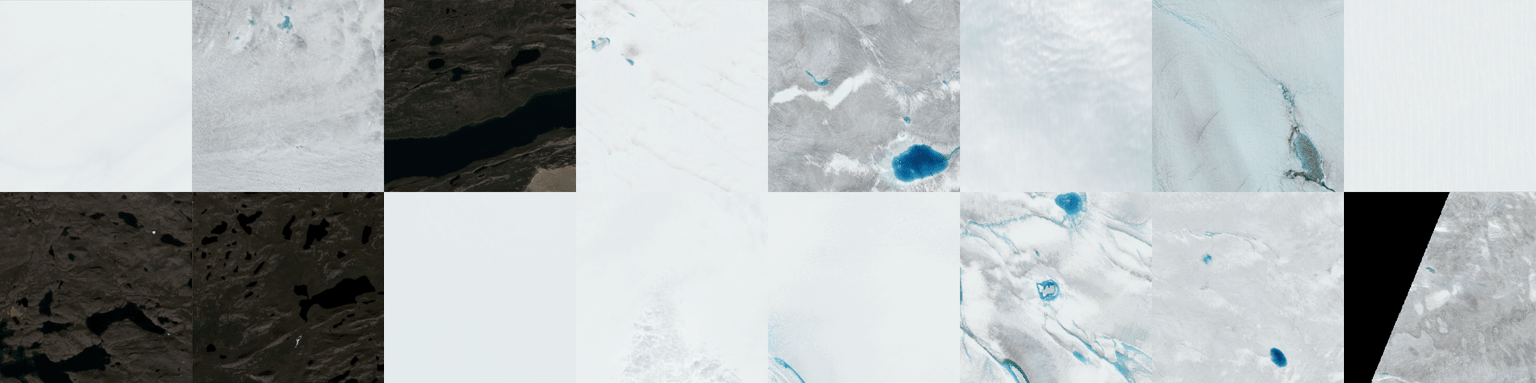
\includegraphics[width=\columnwidth]{images/batch_sample.png}
\caption{Tiles sample}
\small Examples of tiles, with the last one partially extracted at the raster border.
\label{fig:figure1}
\end{figure}


\subsection{Model}
To generate segmentation masks from the image tiles, we used 320x320 RGB image tiles as input for our models to generate binary masks representing the two target classes.
For model training and evaluation, we split the dataset into $80\%$ for training and $20\%$ for validation. 
We trained the final model for submission using the entire dataset.
To help the model generalize, we used the Albumentations\cite{info11020125} library for image augmentation with different kinds of augmentations (rotation, flip, brightness, distortion, \dots).

\subsection{Postprocessing}
To transform the model's predictions into lake polygons, we implemented a two-step postprocessing methodology.
First, we generated predictions by tiling the original raster images with overlap. Subsequently, we aggregated the predicted masks and constructed polygons by identifying their contours.
In the second step, we merged overlapping polygons and filtered them out based on their area.

\section{DeepLabv3+ solution}
\label{deeplabv3}

In this section, we present our DeepLabv3+\cite{chen2018encoderdecoder} architecture, which stands as one of the state-of-the-art models for semantic segmentation \cite{sotasemanticsegmentation}. This solution ranked first in the competition.

\subsection{Preprocessing}

\paragraph{Clustered-based undersampling} We applied a clustering algorithm and used the resulting clusters, with a probability inversely proportional to their size, to randomly select non-lake tiles. This method aims to enhance our chances of selecting tiles that contain important but less common land covers.
The clusters are created using the \textit{k}-means algorithm, with \textit{k} set to $4$ on the histograms of images' HSV color space. We chose a lower number of bins (specifically, $5$ bins per channel) to reduce computation time. The decision for the value of \textit{k} was driven by the intuition that a high \textit{k} would lead to numerous clusters, potentially decreasing the method's efficiency in representing the rarity of land covers. Conversely, a \textit{k} that is too low might capture less disparity between images and leave fewer chances to distinguish the more uncommon images.

\subsection{Model}

\begin{figure}[t!]
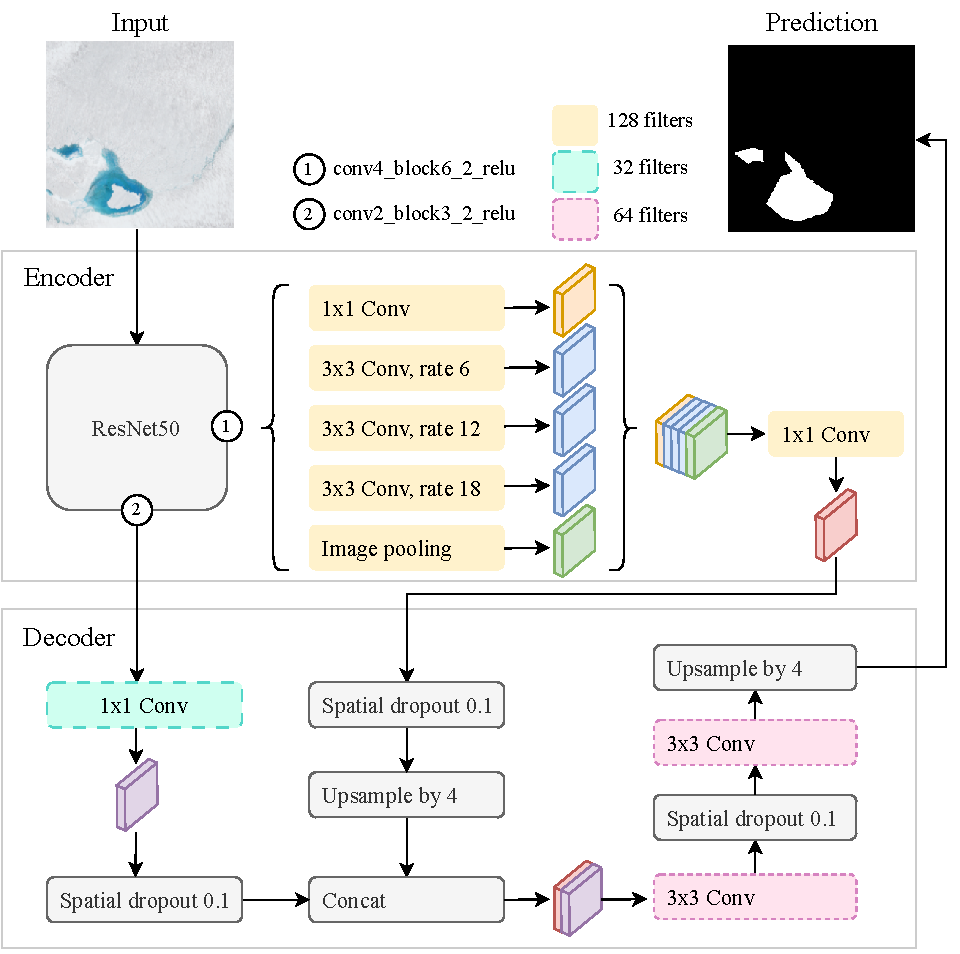
\includegraphics[width=\columnwidth]{images/deeplabv3plus.pdf}
\caption{Modified DeepLabv3+ architecture}
\small Changes include reduced filters and additional spatial dropout layers.
\label{fig:figure2}
\end{figure}

\paragraph{Model architecture} 
We used the DeepLabv3+ example provided on the Keras website\cite{Rakshit} as a basis for our solution and subsequently introduced several improvements to enhance the model's capabilities (see Figure \ref{fig:figure2}). To address concerns related to overfitting and computational efficiency, we chose to reduce the number of filters. This resulted in a model having approximately $20\%$ fewer parameters, totalling 9.5M trainable parameters, as opposed to 11.8M trainable parameters in the original implementation. Additionally, for model regularization, we incorporated three spatial dropout\cite{spatialdropout} layers. In an effort to reduce the model's sensitivity to batch size variations, we replaced batch normalization with group normalization\cite{wu2018group}. Finally, we substituted the conventional ReLU activations with GELU activations\cite{hendrycks2023gaussian}, with the expectation that this change would further enhance model performance.

\paragraph{Training details} The loss function used is a combination of a weighted Binary Cross Entropy (BCE) and Dice loss. By combining both, we benefit from the advantages of Dice loss, notably robustness to class imbalance, while BCE mitigates its drawbacks by smoothing the loss landscape\cite{Jadon_2020}.

\paragraph{Snapshot ensembles} To achieve better performance and ensure a more robust solution, we chose to employ an ensemble of models in this approach. To reduce training time, we created this ensemble following the snapshot ensembles technique\cite{huang2017snapshot}. We trained our models using stochastic gradient descent with the following hyperparameters: a momentum of $0.99$ and a clipnorm of $1$. Additionally, we used a cosine annealing learning rate scheduler\cite{DBLP:journals/corr/LoshchilovH16a} with an initial learning rate set to $0.1$. We determined this initial learning rate through a learning rate range test. The training process is organized into three cycles, each spanning $50$ epochs. At the completion of each cycle, we saved the model weights (see Figure \ref{fig:figure3}). This approach produced three distinct models that constitute the ensemble.

\begin{figure}[t!]
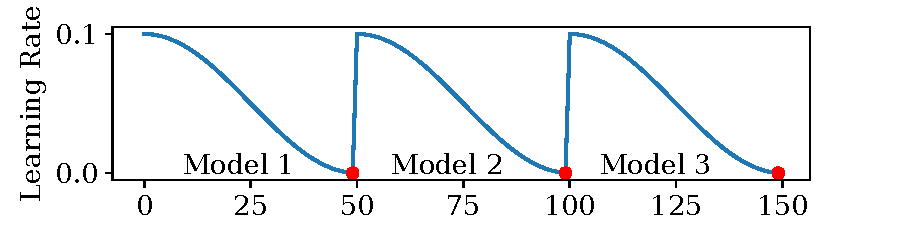
\includegraphics[width=\columnwidth]{images/lr_scheduler.pdf}
\caption{Learning rate scheduler for snapshot ensembling}
\small Weight saving times are marked as red dots.
\label{fig:figure3}
\end{figure}

\subsection{Postprocessing}

\paragraph{Model ensemble} 

To diminish the impact of lake positions in images, which may lead to errors (for instance, when there is a small portion of lakes at the image's borders), and to enhance the robustness of our solution, we made predictions with a three-fold overlap. Since we used three models for predictions, we averaged nine predictions in total, except at the raster's borders where we had a minimum of three predictions.

\section{U-Net solution}
\label{unet}

In this section, we present our U-Net model. This solution ranked fourth in the competition.

\subsection{Preprocessing}

\paragraph{pHash similarity based filtering} We used a perceptual hashing algorithm \cite{idealods2019imagededup} to calculate the hashes of the generated tiles in the preprocessing step. For each image and region, we included all the tiles containing lakes and then selected the ones that did not contain lakes and did not have the same hash. This process ensures that we maintain a consistent distribution of images throughout the images and regions while eliminating similar images.

\paragraph{Dataset bias} Each tile is labelled as either containing a lake or not containing a lake. To create the dataset, we picked a ratio of $0.7$ "lake" to "non-lake" images. As more images were available for training, this introduced a bias in the dataset, predicting fewer lakes, but enhancing the model's robustness to false positives.

\subsection{Model}

\paragraph{Model architecture} We used the U-Net\cite{ronneberger2015unet} encoder-decoder architecture with a pre-trained ResNet50\cite{he2016deep} encoder for predicting the masks. The weights were left trainable with a total of 32.6M parameters. We started with an implementation from NAU-Net\cite{wang2022nau} using the Pytorch Lightning framework.

\paragraph{Training details} We used the Adam optimizer and a custom loss function that combines, in a weighted sum, a Tversky loss ($w_{Tversky}=0.25$) and a custom blob detection loss ($w_{blob}=0.75$) to train the network. The Tversky loss ($alpha=0.6$, $beta=0.4$) is used to ensure that the model is accurate pixel-wise. The blob detection loss is used with the idea of improving the accuracy of the number of predicted lakes. The combination of the two losses allows for more stable training.

We trained the network for $140$ epochs with a batch size of $32$. Through a learning rate range test, we set the learning rate to $0.00015$ and multiplied it by a factor of $0.8$ every $20$ epochs. We incorporate the \textit{StepLR} learning rate scheduler from PyTorch to enhance the model's convergence.

\subsection{Postprocessing}

\paragraph{Edge significance mask}
To enhance the quality of the predictions near tile edges (where lakes may be truncated), we multiplied each one of them with a mask designed to diminish edge significance. We then averaged the predictions over a $50\%$ overlap.
The mask consisted in a $25\%$ border around all edges, set at a value of $0.75$, while maintaining a value of $1.0$ for the inner area.
The border dimensions and value were determined based on the $50\%$ tile overlap. This ensures that overlapping tile edges have a minimum of three confident predictions for annotating border pixels.

\section{Results}

The final evaluation of the submitted geopackage files for lake identification was based on $F_1$-score, which considers precision and recall. Each submitted polygon was to be classified as "true positive", "false positive", or "false negative" in comparison to the withheld test dataset.
As defined by the competition rules, the criteria for a "true positive" includes: no overlap with other polygons in the submitted file, partial or full overlap with a polygon in the test dataset (the predicated area should be between $50\%$ and $160\%$ of the overlapping test area).

The DeepLabv3+ based model ranked first with a $F_1$-score of $0.712$, whereas the U-Net based model ranked fourth with a $F_1$-score of $0.673$.
Using our Linux server (112 cores, 128GB RAM and four NVIDIA A40 graphic cards), computation completes in approximately 8 hours and 4 hours, respectively.

\section{Discussion}
We encountered some noteworthy difficulties with ensuring reliable validation being a particular challenge. Since we employed a random split for validation, there was a possibility of encountering images and their overlaps in both the training and validation datasets. Additionally, it was possible that images taken at the same location but at different times could appear in both the training and validation sets.

To mitigate these issues, we implemented image augmentation. Nevertheless, we found that the metrics we used were not entirely reliable. We noticed that the training and validation Intersection over Union (IoU) were still consistently increasing without any sign of overfitting. It was only when we thoroughly examined the predictions in QGIS that we realized overfitting could still be an issue. We acknowledge that room for improvement exists, particularly in enhancing the model evaluation.

As future endeavour, we could explore the possibilities of combining the various preprocessing and postprocessing methods with the algorithms. This entails
experimenting with different parameters settings. Also, we were unable to dedicate enough time to fully experiment with additional data sources, such as the near infrared channel to implement the Normalized Difference Water Index (NDWI), which has the potential to further enhance lake detection performance. However, it is worth mentioning that our experimentation with gradients computed from ArticDEM as an additional channel did not result in performance improvements. One possible reason is that the DEM model represents the mean average of each image.

These directions are however promising for enhancing the overall performance of our methods.

\section{Guidelines to run the code}
The code of both implementations can be found on GitHub\footnote{https://github.com/swiss-ai-center/giscup2023-deepLabV3Plus} \footnote{https://github.com/swiss-ai-center/giscup2023-resnet-unet} under the MIT license. Refer to the related \emph{README} files to set up the required dependencies, pull data from the remote storage, and run the ML pipeline.

\begin{acks}

We would like to thank Julien Rebetez from \textit{Picterra} and Nils Hamel from \textit{arx iT} for their feedback and suggestions.
This material is based upon work supported by the University of Applied Sciences Western Switzerland (HES-SO) and the Swiss AI Center.

\end{acks}

%%
%% The next two lines define the bibliography style to be used, and
%% the bibliography file.
\bibliographystyle{ACM-Reference-Format}
\bibliography{references}

\end{document}
\endinput
%%
%% End of file `sample-sigconf.tex'.
